\pagenumbering{arabic}

\chapter{Introduction} \label{introduction}

This document provides the Software Specification Requirement (SRS) of an open-source precision agriculture CNC farming project that lets the user grow food from anywhere with a web app. The website for this system is \url{https://farm.bot}

\section{Purpose of the System }

The purpose of the FarmBot system is to revolutionize agricultural practices through automation. FarmBot aims to regularize farming methods, enhance crop yields and minimize resource waste. Additionally; FarmBot provide a platform to manage and monitor their crops and agricultural operations efficiently. Through automation and monitoring, the system aims to:

\begin{itemize}
    \item Automate planting, watering, weeding and harvesting processes to reduce human work and improve efficiency.
    \item Provide precise control over the environmental factors such as soil moisture, harmful weeds.
    \item Facilitate real-time monitoring from web application to enhance crop health.
    \item Provide an environment to design a layout for crops and implement that design in real world.
\end{itemize}

\section{Scope}

In the scope of this system, Farmbot is humanity's open-source CNC farming machine that automatically grows food right in your backyard keeping you in complete control, as opposed to the current food production system which no longer has control over how the food is produced. 

\begin{itemize}
    \item Farmbot is provided with 95 pre-assembled elements to be set up quickly and easily and perform the basic functions needed to grow a garden.
    \item Raspberry Pi computers operate the system with its hardware components (webcam, Arduino firmware microcontroller combined with powerful stepper motors and dynamic devices, ph sensors) and user application requests.
    \item Farmduino microcontrollers allow positioning of the tool head with millimetre accuracy for sowing, and watering plants in any pattern and frequency with given built-in features of plants based on their type, age, and soil conditions. The sensors also send the condition of soil and weather data of pH, temperature, and moisture.
    \item The Onboard camera system allows user to monitor their garden, and capture images, and the farmbot can take action by detecting the weeds utilising advanced computer vision.
    \item The web and mobile application allows users to control the garden remotely, and configure or update the software of Raspberry Pi computers without any need for hardware change.
    \item The farm designer and sequence editors allow users to lay out their plants with built-in data for plants, creating optimal layouts each season, and taking care of their plants in the way they want without requiring any coding.
    \item The farmbot software development allows professionals to modify and use it for any purpose (e.g. education, business) in hardware tools or develop completely new versions of the farmbot based on the existing library of components.
\end{itemize}

\section{System Overview}

This section of the document will provide detailed information about the system
including all components.

\subsection{System Perspective}

\begin{figure}[h!]
  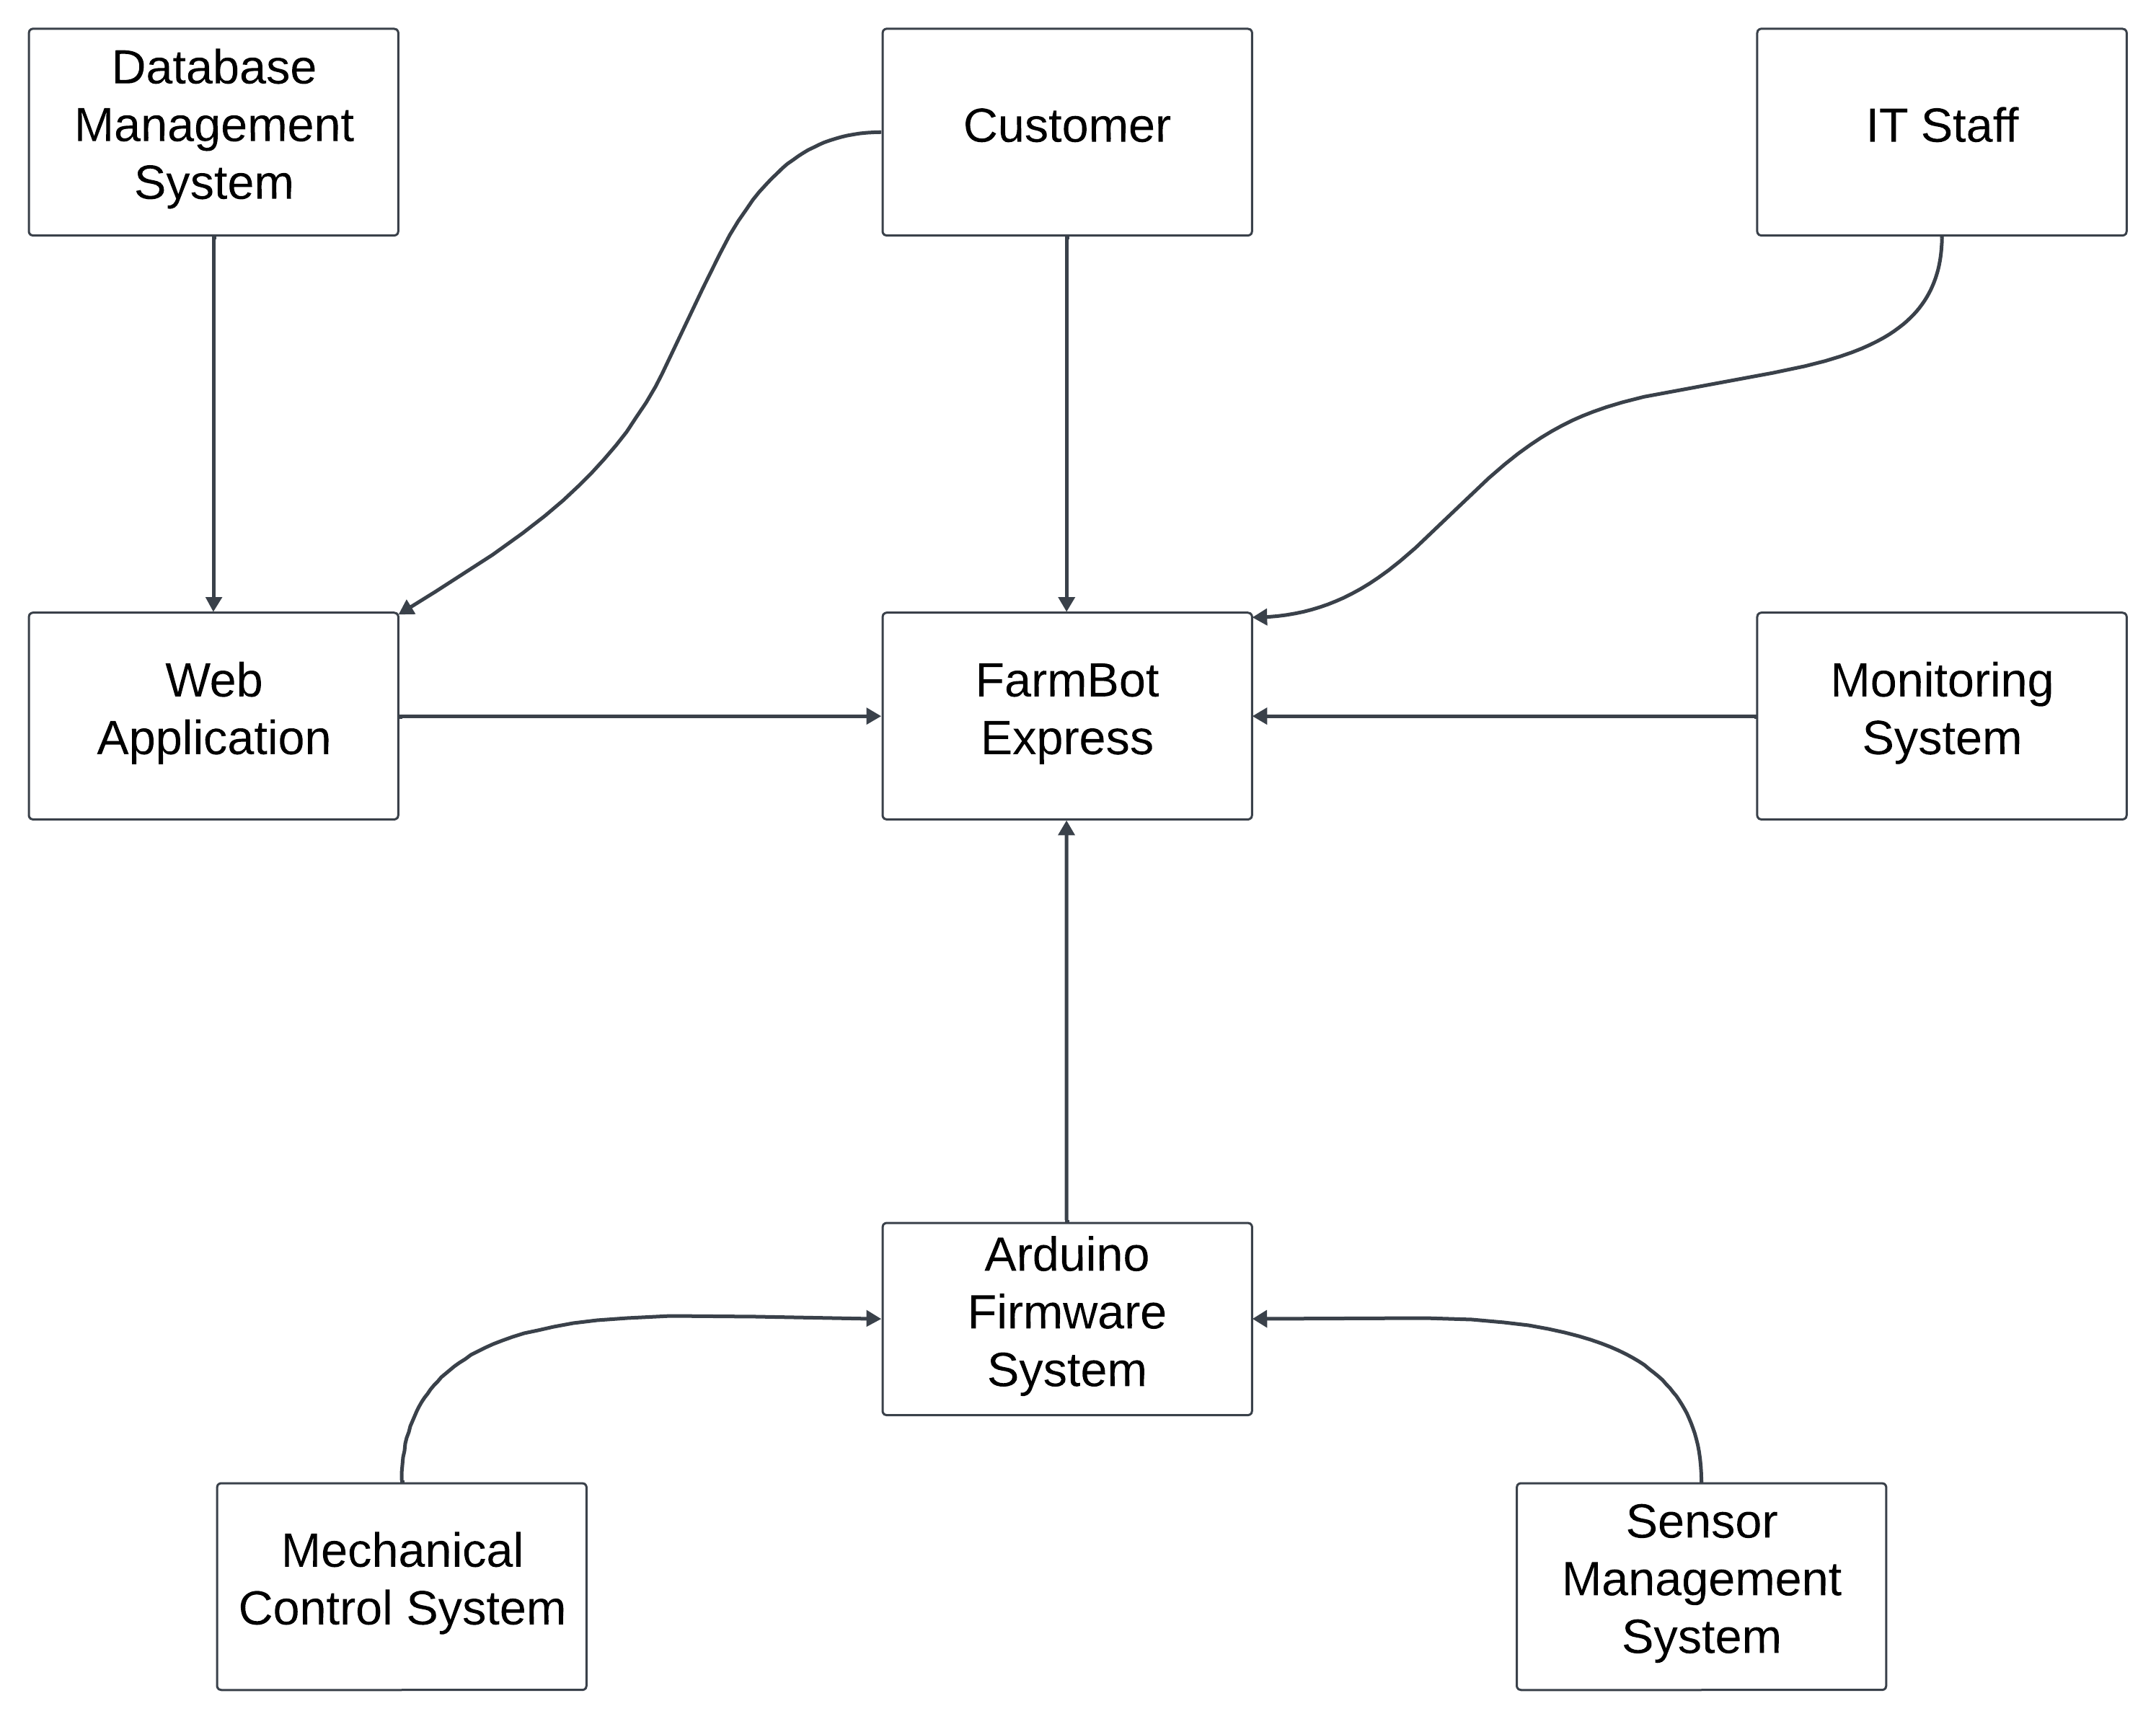
\includegraphics[width=\linewidth]{Figures/context-diagram.png}
  \caption{Context Diagram of FarmBot Express}
\end{figure}

\newpage

FarmBot is not part of a large system nor necessarily requires the download of an application. Hence customers shall go into the web browser of the app and configure their FarmBot using their laptop, tablet, or smartphone.
The web application features real-time manual controls and logging, a sequence builder for custom routines for FarmBot to execute.The web application keeps the data and receives the built-in data for plants from the database management system. The machine maintains a connection and synchronises with the web application via the message broker. Besides that, Farmbot communicates with the Arduino firmware system over a serial connection to send commands for motor and tool positioning and receive collected from sensors and rotary encoders. Moreover, the FarmBot is connected to a monitoring system through a webcam to provide real-time view, image-capturing, and detecting weeds, taking actions according to it. Furthermore, the system provides an IT staff interface in case of loggings, errors and customary configurations to help customers.


Refer to \textit{(Clause 9.6.4, 9.5.4.1)}
\subsubsection{System Interfaces}

\begin{itemize}
    \item \textbf{Monitoring System:} In the FarmBot Express, the camera is provided within the kit. The kit is connected to Raspberry Pi through a USB cable or serial connection. The monitoring system receives data from the camera and using built-in computer vision functions, it detects the weeds and layout of the garden in general. According to the status of the garden, it takes actions autonomously or alerts the customer through the web application using the MQTT Gateway service. Moreover, it provides a real-time view or image-capturing from recorded data.
    
    \item \textbf{Arduino Firmware System:} The system consists of two subsystems named Mechanical Control System and Sensor Management System. The firmware that is flashed onto the Arduino or Farmduino microcontroller is responsible for physically operating FarmBot’s motors, tools, sensors, and other electronics. It receives G and F codes from FarmBot OS, and then moves the motors and reads and writes pins accordingly. It also sends collected data from the rotary encoders and pin reads back to the Raspberry Pi. The processed data returns as a command from the main system to position tool heads to set light, sow weeds, and water plants.

    \item \textbf{Mechanical Control System:} This system is primarily constructed from V-slot aluminium extrusions and aluminium plates and brackets. They are driven by four NEMA 17 stepper motors, the Farmduino Express microcontroller, and a Raspberry Pi Zero 2 W computer.
    The bots roll directly on the wood-raised bed. FarmBot Express features a three-in-one tool head and does not require any additional precision tool. The gantry allows the tool head to be moved in the X-direction and serves as a guide for the Y and Z directions. The gantry also supports the structure for mounting the electronics box and seed troughs.
    
    \item \textbf{Sensor Management System:} This system has soil moisture, temperature, light, pH, humidity, and weather sensors. The abrupt measurements are sent to the Farmduino Express microcontroller. The firmware and Raspberry Pi computers process data and take actions autonomously
    or if it requires further investigation, it sends messages to the web server.

    \item \textbf{Web Application:} This system allows users to control and configure their FarmBot from most electronic devices. It does not require installation since it is a web-based application. The core features include the farm designer, event scheduler, sequence editor, regimen editor, controls, management of FarmBot's tools and seed containers, management of FarmBot's settings, storage and viewing of logs and sensor readings. Moreover, the application cloud is connected to the crop database.

    \item \textbf{Database Management System:} This system serves as a comprehensive repository of information about botanics and personal gardens. The general built-in data details are planting information, growing requirements, watering needs, nutritional needs, companion planting, pest and disease management, and harvesting and maintenance. Overall, the crop database is a valuable resource for users, so that they do not have to search for plants or to be experts.
    
\end{itemize}

\subsubsection{User Interfaces}
<<<<<<< Updated upstream
Refer to \textit{(Clause 9.6.4.2)}
=======

FarmBot Express users and IT staff interact with the system primarily through a web-based application accessible via computer and mobile device browsers. The interface facilitates various functionalities essential for managing and monitoring farm operations. Furthermore; embedded operating system of the FarmBot Express is also available as open-source code. So a customer or an IT member can access the operating system code and configure the embedded system of the FarmBot Express by using means of embedded microcontroller chip. The following parts constitute the user interface:

\begin{itemize}
    \item \textbf{Customer Interface: } Users are required to create an account by providing necessary details such as name, email address, and password. After signing, users can log in using their credentials to access their accounts.
    Upon logging in, users are greeted with a dashboard displaying key information such as current garden layout, planted crops and real photos of the layout. The dashboard provides tabs of the farming operations that allow users to navigate to different sections of the application. These tabs can be grouped as below:
    	\begin{itemize}
 	   \item \textbf{Layout Screen: } Shows the layout of the garden. It shows real photos of the garden, harmful weeds, the spread area of the planted crops, condition of the soil etc. directly on the garden layout.  
    	   \item \textbf{Plants: } In this tab, user can view and manage all of the plants in the garden. Plants can be dragged and dropped to the garden layout to make a design.
    	   \item \textbf{Weeds: } This tab stands for viewing and managing the weeds in the garden. Weeds that are detected by FarmBot Express appear in this tab. User can select which weeds to be removed and what is the period of the removal.
    	   \item \textbf{Points: } This tab provides information about soil in the different point of the garden. User can select points to monitor soil condition.
    	   \item \textbf{Curves: } This tab provides information about water, spread and height curves for the plants. User can determine amount of water, spread and height of the plants in this tab.
    	   \item \textbf{Sequences: } In this tab, user can configure sequences by putting some steps in order like first plant the seed, water it and then take a photo of it.
    	   \item \textbf{Regimens: } This tab stands for scheduling sequences based on the age of the plants.
    	   \item \textbf{Events: } This tab provides an overview of schedulend sequences and regimens for the user.
    	   \item \textbf{Sensors: } This tab provides information about historical sensor readings. It also allows user to view current sensor readings and manage sensors.
    	   \item \textbf{Phoros: } In this tab, user can view and manage photos of the garden taken by FarmBot Express. It also allows user to calibrate camera and weed detection settings of the FarmBot Express.
    	   \item \textbf{Tools: } This tab allows user to view detailed information about and manage tools, seed containers, and slots in the garden. 
    	   \item \textbf{Messages: } This tab includes messages and announcements for the user.
    	   \item \textbf{Help: } In this tab, user can see the documentation of the web-application and can get support from IT members.
    	   \item \textbf{Settings: } This tab is the settings tab for web-application. Mainly for configuring accounts of the user.
    	   \item \textbf{Contols: } This tab provides a controller interface for user to control movements of FarmBot Express manually.
    	   \item \textbf{Jobs and Logs: } In this tab, user can view running and completed jobs.
    	   \item \textbf{Connectivity: } This tab provides information about the connection between the web browser, FarmBot Express, and the FarmBot web-application servers.
	\end{itemize}
	
	Besides this web-application user interface,  the web-application and the embedded operating system of the FarmBot Express are open-source. So advanced users can configure the application and operating system as they want. Last thing to mention is that, FarmBot provides a REST API to edit information such as sequences and the gardan layout without using web-application directly.
	
	\item \textbf{IT Staff Interface: } While there isn't an interface exclusively designed for IT staff within the FarmBot Express system, IT members have access to the source code of both the web-application and the embedded operating system of the FarmBot Express as they are open source. This access enables them to support users and perform configurations as needed.
\end{itemize}
	





>>>>>>> Stashed changes
\subsubsection{Hardware Interfaces}

The system requires a borescope camera, Raspberry Pi computer, Farmduino, several sensors, four motors, rotary encoders, Vacuum Pump, audio jack, micro SD Card, Wi-Fi radio antenna, Ethernet connector, several USB cables, UTM cable, power supply, LED light strip, water solenoid valve and the universal tool mount. The camera supports advanced computer vision technologies. The Raspberry Pi computer, Farmduino and many mechanical devices are usually connected through USB cables. To receive data and send commands, the vacuum pump, water solenoid valve, encoders, motors, and light strip are integrated into the Raspberry Pi. Another hardware requirement is an electronic device that has a connection to the web server. Hence the Ethernet connector or the Wi-fi radio antenna must be implemented into the Farmduino firmware. Overall, the Raspberry Pi serves as a communication node between the Web App and the Farmduino via message broker, MQTT gateway. This communication allows Raspberry Pi to get instructions, customary configurations, and modifications manually from the web app to the Farmduino and hence to other hardware products.


\subsubsection{Software Interfaces}
\begin{itemize}
	\item \textbf{Database: } OpenFarm which is a free and open source database for farming and gardening knowledge is used for this service. This service stores and provides crop and growing information to the web app for a streamlined user experienced. Any information in the tabs mentioned in the \hyperref[subsubsection.1.3.1.2]{User Interface} stored in the database. This information includes data accumulated by the sensors of the FarmBot Express such as moisture of the soil, temperature; data obtained from the photos provided by the webcam of the FarmBot Express such as weeds in the garden; data related to planned garden layout; data of jobs and scheduled sequences and much more. 
	\begin{itemize}
		\item Name: OpenFarm
		\item Version Number: Last stable version
		\item Source: \url{https://openfarm.cc/}
	\end{itemize}
	
	
\end{itemize}


\subsubsection{Communication Interfaces}

The communication protocol between FarmBot Express and the web application is established using the MQTT Gateway protocol. MQTT is a lightweight messaging protocol ideal for communication between constrained devices and network servers. MQTT operates on a publish-subscribe messaging pattern, allowing FarmBot Express and the web application to exchange messages asynchronously. Messages are published by either FarmBot Express or the web application and subscribed to by the respective counterpart to facilitate bidirectional communication. The message content includes commands, sensor readings, job logs, data obtained by the hardware and photos taken by the webcam.

\subsubsection{Memory Constraints}

The system's application is web-based, therefore there is no requirement to have storage in the user's device. On the other hand, the Farmbot Express is a microcontroller after all, hence it has built-in preserved area storage for program and data memories. Hence there is a memory constraint to keep webcam images, recordings, and data of several sensors. The data should be sent to web cloud services before overwriting. Moreover, it is an open-source system, hence the functions, OS and more can be configured by customers which affects the preserved program memory. 

\subsubsection{Operations}
Refer to \textit{(Clause 9.6.4.7)}

\subsection{System Functions}

Refer to \textit{(Clause 9.6.5, 9.5.4.2)}. If you want to add any figure or diagram, you can use a figure environment.In Figure \ref{Fig:Example}

\begin{figure}[ht]
\centering
\includegraphics[width=.9 \textwidth]{Figures/ExampleFigure.png}
\caption{Example \label{Fig:Example}}
\end{figure}


\subsection{Stakeholder Characteristics}

Refer to \textit{(Clause 9.6.6, 9.5.4.3, 9.4.5)}

\subsection{Limitations}

Refer to \textit{(Clause 9.6.7)}

\section{Definitions}

You should add acronyms and abbreviations here. Refer to \textit{(Clause 9.6.7)}



For any citation, refer to it as \cite{younis2021hybrid}.
